% a_zer_rename_committer.tex
\documentclass[conference]{IEEEtran}
%\usepackage{babel}
\usepackage{graphicx}
\usepackage{color}
\usepackage{cite}
%\usepackage{algorithmic}
%\usepackage{algorithmicx}
\usepackage[ruled,vlined]{algorithm2e}
\usepackage{listings}
%\usepackage{minted}
\usepackage{underscore}
\usepackage{multicol}
\usepackage{float}
\usepackage{checkend}
\usepackage{enumitem}

% ========================================================================
% commands


\newcommand{\SUCCESS}{\texttt{\_SUCCESS}}

% add a todo marker. We can turn this off when we don't want to see it.
\newcommand{\TODO}{\emph{TODO}}
% ========================================================================


\title{
A Zero-Rename Committer:\\
Object-storage as a destination for Apache Hadoop and Spark}

% Yes, this titling is broken
\author{
  Loughran, Steve
  \texttt{stevel@hortonworks.com}\\
\and
  Blue, Ryan
  \texttt{rblue@netflix.com}\\
\and
  Radia, Sanjay
  \texttt{sanjay@hortonworks.com} \\
\and
  Balamohan, Rajesh
  \texttt{rbalamohan@hortonworks.com} \\
}

\date{December 2017}

% ========================================================================

\begin{document}


\maketitle

% ========================================================================

\begin{abstract}

We introduce new \emph{committers} for Apache Hadoop, so permitting
the Amazon S3 Object Store to be used as a direct destination of output generated
by Hadoop MapReduce and Apache Spark.

By using the operations directly exported by
the store, most critically the multipart upload mechanism, these committers upload
their output to the final destination, yet do not materialize this data until the
overall job is committed.
As a result, the committers meet the core requirement of the Hadoop and Spark commit
protocols: output is not visible until committed, while being highly-performant.

We also define the commit protocols of Hadoop and Spark, and show how the classic committer
implementation's requirements of atomic file creation and rename operations mean that they
cannot be safely used with Amazon S3.
hus the new committers are not just ``better'' committers for object stores,
but fundamentally safe for use.

We discuss the two committers, ``Staging'' and ``Magic'', exploring their differences.
The Staging committer stages all generated output to the local filesystem of
worker nodes, uploading this data when a task is committed.
The Magic committer streams data directly to the object store, relying on the
object store client to recognise some output paths as special (``magic''), and
so translating writes to these paths as initiating a delayed-completion write
to a calculated final destination.

\end{abstract}

% ========================================================================

\section{Introduction}
\label{sec:introduction}

It has long been a core requirement of ``Big Data'' computation platforms that
the source and destination of data was a fully consistent distributed filesystem,
albeit often ``sub-POSIX''.

Distributed, because data needs to be readable and writeable by all processes
executing a query across the cluster of computers.
``Sub-POSIX'', in that the full semantics of the POSIX filesystem APIs were not always necessary.
A commonly dropped requirement is the ability to seek past the end of the file and
write data, with a secondary dropped behavior one of being able to overwrite existing
data within a file.
That is: new data could only be written at the current end of the file.
What has been a consistent part of the required semantics has been that the filesystem
presents a model of directories and files with consistent operations to list and
read those directories, and at least four atomic operations:

\begin{itemize}
  \item rename of a single file to another location within the same volume 
  \item rename of a directory and its contents to another location within the same volume 
  \item create file with no overwrite 
  \item recursive delete of a directory 
\end{itemize}

These operations are often used as the foundational operators of higher-level
co-ordination and commit protocols.

For example, the \texttt{create()} operation can be used to obtain a lock on a resource:
the first process to create a file can consider itself having exclusive access to it,
and so implicitly consider itself to have acquired the resource.

The \texttt{rename()} operation is generally critical to providing atomic promotion
of output: a single \texttt{rename()} call can promote all in-progress output
of a worker to become completed work, simply by moving all the output to a well known path.
And, when the job completes, its final output may be renamed to a new location to become
publicly visible.

As covered in\ \cite{MapReduce}:

\begin{quote}
We rely on the atomic rename operation provided by the underlying file system
to guarantee that the final file system state contains just the data produced
by one execution of the reduce task.
\end{quote}


Apache Hadoop was written with its own filesystem, Hadoop Distributed File System (HDFS).

It is self-admittedly ``sub-POSIX'', specifically, while presenting the POSIX
model of a filesystem tree containing directories and files, data can only be
appended directly to the end of the current file.
That is: one my not \texttt{seek()} to before or after the end of the file and
then write data.

It does offer atomic operations which are used in commit protocols and other
applications as a means of enforcing exclusivity;
so permitting the filesystem to act as a mechanism of co-ordinating access across machines.

% ========================================================================

\section{The Hadoop MapReduce Commit Algorithm}
\label{sec:commit}


\subsubsection{Terminology}

First, some terminology needs to be introduced to describe
the protocols.


\textbf{Job}.
A parallelized query/operation to execute.

The output of a Job is made visible to other stages in a larger operation
sequence or other applications if the job \emph{completes successfully}.

\textbf{Job Attempt}.
A single attempt at executing the job;
each one executed from a new set of processes.
Hadoop Jobs are restartable, so more than one attempt may be made;

\textbf{Task}.
A single operation within a job, on a single process, one which generates
one or more files.
A task completes successfully if it generates all the output it expects to without
failing in some way.

\textbf{Task Attempt}.
A single attempt to execute a task.
Multiple attempts may be made to execute a task;
possibly in parallel.
It is critical that only one task attempt's output is propagated
to the final output of a job.


\textbf{Job Manager}.
Whatever process schedules
task execution, tracks success/failures and, determines when all the work has been
processed and then commits the output.
It may also determine that a job
has failed and cannot be recovered, in which case the job is aborted.
In MR and Tez, this is inside the YARN application master.
In Spark it is the ``Spark Driver'', which can be executed in a number of
locations, including the same process as that in which the tasks are executed.


\textbf{Executor}.
A process capable of executing work, as directed by the Job Driver.
In Hadoop, a unique

\textbf{Final directory}.
The directory into which the output of a job is placed
so as to be visible.
After a successful job completion, the data MUST be visible in the final directory.


\textbf{Job Context}.
An instance of the class \texttt{org.apache.hadoop.mapreduce.JobContext},
which provides a read-only view of the Job for the Job Driver and tasks.

\textbf{Task Attempt Context}.
an instance of the class
\texttt{org.apache.hadoop.mapreduce.TaskAttemptContext},
which provides operations for tasks, such as getting and setting status,
progress and counter values.

\textbf{Task Working Directory}.
A directory for exclusive access by a single task,
into which uncommitted work may be placed.

\textbf{Task Commit}.
The act of taking the output of a task attempt and promoting it
to become part of the final output of the active job
attempt.

\textbf{Job Commit}.
The act of taking the output of all committed tasks of a job attempt,
and generating the final output.
This normally consists of publishing this output in an aggregate form;
it can also include generating extra summary data.
As this it is often a serialized operation at the end of a job attempt,
its performance can be a bottleneck.

\textbf{Task Abort}.
To cancel a task such that its data is not committed.

\textbf{Job Abort}.
To cancel all work in a job attempt: no task's work is committed.


\subsection{Requirements of a Commitment Protocol}
\label{subsec:requirementsOfACommitmentProtocol}

Apache Hadoop's MapReduce implementation is designed to support long-lived
large-scale queries taking minutes to hours to complete.
Its requirements include the following:

\begin{enumerate}

  \item Support thousands to tens of thousands of invidually scheduled $tasks$
  within a single $job$.

  \item Support different destinations of work, such as filesystems and databases.

  \item Recover from the failure of a task attempt by rescheduling the task;
  a new task attempt may be executed anywhere within the cluster.

  \item Support speculative execution of task attempts as a means of compensating for the
  delay caused by \emph{stragglers} in the execution.

  \item Potentially: recover from a failure of a job attempt, using all the committed
  task output from the previous, failed attempt.

  \item Be resilient to network failures/partitions of tasks, and of the job manager
  itself becoming isolated from other parts of the system (and hence: a second
  attempt at the job being started).

\end{enumerate}

This leads to some specific requirements of the implementation, requirements
which can be used to assess the correctness of the implementation.

\textbf{Independent.}
Individual tasks must be able to write their data without directly
co-ordinating that write with those of other tasks.

\textbf{Speculative tasks until committed.}
Multiple tasks must be able to simultaneously execute on the same input
source, to generate the required output of that part of the input.
This is required for recovery, and for speculation.
Non requirement: idempotent output;
that is left to the implementors of the operations executed in the tasks.

\textbf{Scaleable communication protocol.}
The commit protocol communications between task and job manager
must be efficient enough to support tens of thousands of simultaneous
tasks.

\textbf{Abortable.}
It must be possible to abort an uncommitted task or job.
There should be no leftover output.

\textbf{Recoverable or Restartable Job.}
A committer can declare whether or not it supports job recovery;
if it does, it must implement recovery.
If not, the job must be restartable from the beginning.

\begin{figure*}
  \centering
  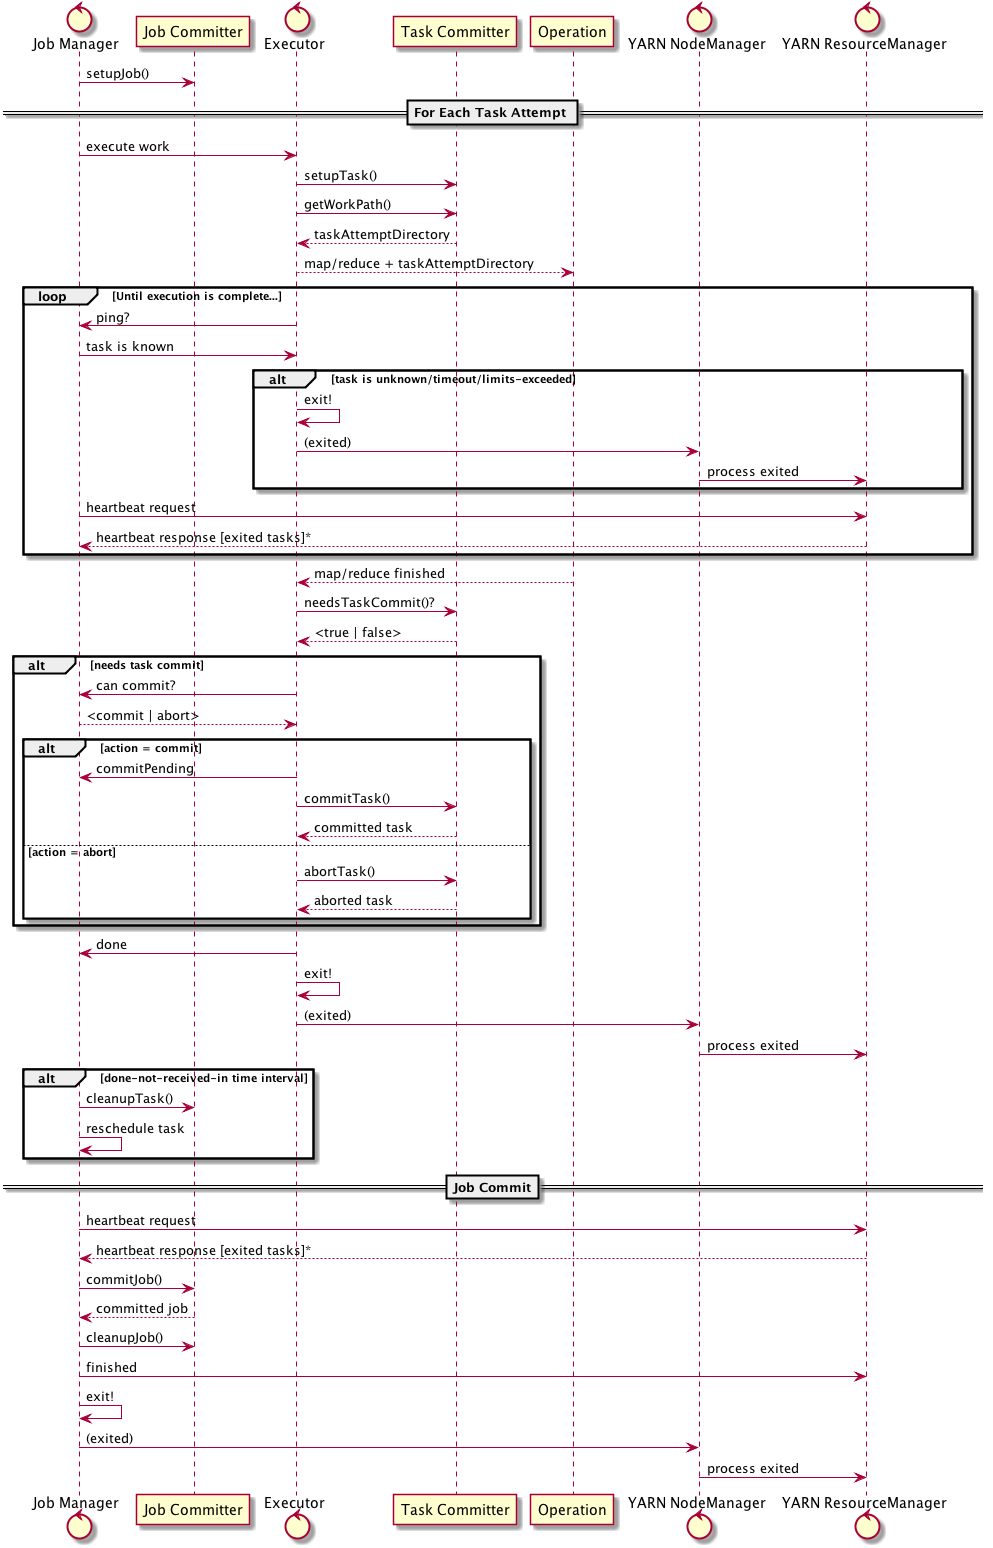
\includegraphics[width=.8\textwidth]{commit-protocol.png}
  \caption{Hadoop commit protocol (excluding Job recovery)}
  \label{fig:commit-protocol}
\end{figure*}

An UML sequence diagram of the core commit protocol is
show in\ \ref{fig:commit-protocol}.

The commit algorithm is designed to work on the YARN cluster scheduler
\ \cite{Vavilapalli2013}.
This launches the initial Application Master, containing what we call
the ``Job Driver'', and any processes requested by the Application Master
(``the AM'').
On each node in the YARN cluster, a \emph{NodeManager} has the responsibility
of launching the applications, usually within a memory-and-CPU-bounded
environment.
When a launch process terminates, this fact, and the process exit code
is passed to the \emph{ResourceManager} within the regular status heartbeats
between each NodeManager and the ResourceManager.
The ResourceManager passes this information on to the Application Master
as part of the regular heartbeat in the ``AM/RM protocol''.

% -----------------------------------------------------------------------

\subsection{Optional recoverable failure modes}
\label{subsec:optionalRecoverableFailureModes}

\subsubsection{Job Recovery}
The second Job driver process queries the Job Committer as to whether job
recovery is supported.
A committer can declare whether or not it supports job recovery;
If it does, it must implement recovery on a task-by-task basis;
all tasks which have not been executed or successfully recovered will be
re-run.
If job recovery is not support the entire job is re-executed.

\subsubsection{Bad Records}

Omitted: map/reduce failure from bad data

To avoid an entire job failing due to a single unprocesseable records,
there is an option to skip records whose processing raises an exception.
If the number of failures in a map or reduce operation is below a given
threshold, these records will not result in a task reporting itself as
having failed.
This is not of direct relevance to the commit protocol.


\subsubsection{Hadoop's FileOutputCommitter}

The operations to commit the work, the Task Committer and Job Committer,
are all implemented in the same class, an implementatipon of \texttt{OutputCommitter}.
For writing to HDFS, this is done in the \texttt{FileOutputCommitter}.

This actually implements two separate algorithms for committing work

The longer a job takes to execute, the higher the probability that the (single)
job manager will fail, and hence the ability to recover from a job failure
considered valuable.


Jobs which take a few minutes are generally so inexpensive to
restart that focusing on execution time over recoverability is a better strategy.

For this reason, Hadoop's \texttt{FileOutputCommitter} implements two
different commit algorithms, the purer "V1" and more robust algorithm and the
faster "V2" algorithm.


\textbf{V1.}
Task commit promotes work to a job attempt directory;
job commit promotes this to the destination.
A restarted job can enumerate all work (atomically)
committed by tasks and reuse this output.

\textbf{V2.}
Tasks commit their output direct to the destination directory.
A restarted job must delete the contents of this directory and reexecute
the entire job.

\begin{table}
  \caption{Attributes of the \texttt{FileOutputCommitter} algorithms}
  \begin{tabular}{ l c c }
    \hline
    & \textbf{v1} & \textbf{v2} \\
    Independent & True & True \\
    Speculative Tasks & True & True \\
    Recoverable Job & True & False \\
    Abortable Job & True & Delete output directory \\
    Observable & False & True \\
    Atomic Task Commit & True & False \\
    Idempotent Task Commit & True & False \\
    Atomic Job Commit & False & True \\
    Idempotent Job Commit & False & True \\
    \hline
  \end{tabular}
  \label{tab:file-committer-attributes}
\end{table}


\subsection{Hadoop V1 commit algorithm}
\label{subsec:hadoopV1CommitAlgorithm}


\textbf{Job Setup}

This creates the path \emph{jobAttemptPath}, under the
directory \texttt{\_temporary} of the destination directory
\emph{destPath}.

\begin{procedure}
\caption{setupJob()}
\SetKwData{fs}{fs}
\SetKwData{taskCommittedPath}{taskCommittedPath}
\SetKwData{taskAttemptPath}{\$taskAttemptPath}
\SetKwData{jobAttemptPath}{\$jobAttemptPath}
\SetKwData{jobAttemptId}{\$jobAttemptId}
\SetKwData{taskAttemptId}{\$taskAttemptId}
\SetKwData{dest}{\$destDir}
\SetKwData{temp}{\_temporary}
\SetKwData{SUCCESS}{\_SUCCESS}

% Operations, which are defined for all subsequent procedures/functions
\SetKwFunction{exists}{exists}
\SetKwFunction{delete}{delete}
\SetKwFunction{getFileStatus}{getFileStatus}
\SetKwFunction{isDirectory}{isDirectory}
\SetKwFunction{isFile}{isFile}
\SetKwFunction{listFiles}{listFiles}
\SetKwFunction{mergePaths}{mergePathsV1}
\SetKwFunction{mkdir}{mkdir}
\SetKwFunction{mkdirs}{mkdirs}
\SetKwFunction{rename}{rename}
\SetKwFunction{touch}{touch}
\SetKwFunction{commitJob}{commitJob}

jobAttemptPath := \dest/\temp/\jobAttemptId\;
  \mkdir(\fs, \jobAttemptPath)\;
\end{procedure}

Note Hadoop has a convention that all paths starting with ``\_'' are not considered
``visible'';
everything under this directory is excluded from normal
listings of the destination path.
Creating all intermediate files in a subdirectory of the destination
directory provides an implicit guarantee that the data is created in the
same volume (in a multi-volume filesystem), and in the same encryption zone,
for any HDFS cluster with encryption enabled.


\textbf{Task Setup}

The task attempt is given

\begin{procedure}
%\SetAlgoLined
\caption{setupTask()}
\SetKwData{fs}{fs}
\SetKwData{taskCommittedPath}{taskCommittedPath}
\SetKwData{taskAttemptPath}{\$taskAttemptPath}
\SetKwData{jobAttemptPath}{\$jobAttemptPath}
\SetKwData{jobAttemptId}{\$jobAttemptId}
\SetKwData{taskAttemptId}{\$taskAttemptId}
\SetKwData{dest}{\$destDir}
\SetKwData{temp}{\_temporary}


taskAttemptPath := \jobAttemptPath/\taskAttemptId\;
\end{procedure}

None: directories are created on demand.


\textbf{Needs Task Commit}

The commit is required iff data was generated

\begin{function}
\caption{needsTaskCommit()}
\SetKwData{fs}{fs}
\SetKwData{taskCommittedPath}{taskCommittedPath}
\SetKwData{taskAttemptPath}{\$taskAttemptPath}
\SetKwData{jobAttemptPath}{\$jobAttemptPath}
\SetKwData{jobAttemptId}{\$jobAttemptId}
\SetKwData{taskAttemptId}{\$taskAttemptId}
\SetKwData{dest}{\$destDir}
\SetKwData{temp}{\_temporary}


\exists(\fs, \taskAttemptPath)\;
\end{function}

This is a common place where listing inconsistencies will surface.


\textbf{Task Commit}

Rename task attempt path to task committed path.

\begin{procedure}
%\SetAlgoLined
\caption{commitTask()}
%\KwResult{how to write algorithm with \LaTeX2e }
\SetKwData{fs}{fs}
\SetKwData{taskCommittedPath}{\$taskCommittedPath}
\SetKwData{taskAttemptPath}{\$taskAttemptPath}
\SetKwData{jobAttemptPath}{\$jobAttemptPath}
\SetKwData{jobAttemptId}{\$jobAttemptId}
\SetKwData{taskAttemptId}{\$taskAttemptId}
\SetKwData{dest}{\$destDir}
\SetKwData{temp}{\_temporary}

\If{\exists(\fs, \taskAttemptPath)} {
  \delete(\fs, \taskCommittedPath, recursive)\;
  \rename(\fs, \taskAttemptPath, \taskCommittedPath)\;
}
\end{procedure}


In a file system, this is an $O(1)$ atomic operation.
Even if the task fails to report to the Job Driver that the
commit operation was completed, the existence of the \texttt{taskCommittedPath}
is an implicit confirmation that the task was committed.
Its absence is not a guarantee that the task has failed ---it could just
be taking slow to execute the operation.
However, the Job Driver can assume that the task has failed,
and reschedule another attempt at that task.
Whichever of the rescheduled or original (delayed/partitioned) task
first renames their attempt to the committed path will block the other
from renaming its own attempt directory the same committed task path.

Thus it is not merely the atomicity of the directory rename operation
which the algorithm depends upon, it is the exclusivity.
Only one task attempt from a set of task attempts may rename its attempt to
final path.

\textbf{Task Abort}

Delete task attempt path.

\begin{procedure}
\caption{abortTask()}
  %\KwResult{how to write algorithm with \LaTeX2e }
\SetKwData{fs}{fs}
\SetKwData{taskCommittedPath}{taskCommittedPath}
\SetKwData{taskAttemptPath}{\$taskAttemptPath}
\SetKwData{jobAttemptPath}{\$jobAttemptPath}
\SetKwData{jobAttemptId}{\$jobAttemptId}
\SetKwData{taskAttemptId}{\$taskAttemptId}
\SetKwData{dest}{\$destDir}
\SetKwData{temp}{\_temporary}

  \delete(\fs, \taskAttemptPath, $recursive$)\;
\end{procedure}


On a genuine fileystem this is an $O(1)$` operation.
On an object store, usually $O(files)$.


\textbf{Job Commit}

Merge all files/directories in all task commited paths into final destination path.
Optionally;
create 0-byte `\SUCCESS` file in the destination directory.

\begin{procedure*}
  \caption{commitJob()}
  %  \SetAlgoLined
  \SetKwData{fs}{fs}
  \SetKwData{taskCommittedPath}{taskCommittedPath}
  \SetKwData{taskAttemptPath}{\$taskAttemptPath}
  \SetKwData{jobAttemptPath}{\$jobAttemptPath}
  \SetKwData{jobAttemptId}{\$jobAttemptId}
  \SetKwData{taskAttemptId}{\$taskAttemptId}
  \SetKwData{dest}{\$destDir}
  \SetKwData{temp}{\_temporary}
  \SetKwData{SUCCESS}{\_SUCCESS}

%\KwResult{how to write algorithm with \LaTeX2e }
  \For {committedTask $\leftarrow$ listFiles(\fs, \jobAttemptPath)} {
    \mergePaths(\fs, committedTask, \dest)\;
  }
  \touch(\fs, \dest/\SUCCESS)\;
  \delete(\fs, \temp)\;
\end{procedure*}

% ------------------------------------------------------------
\begin{procedure*}
\label{alg:mergePathsV1}
\caption{mergePathsV1(fs, rc, dest)}


\eIf {\isFile(fs, src)} {
  \If {\exists(fs, dest)} {
    \delete(fs, dest, recursive)\;
  }
  \rename(fs, src, dest)\;
} {
  \eIf {\exists(fs, dest)} {
    \eIf {\isFile(fs, dest)} {
      \delete(fs, dest, recursive)\;
      \rename(fs, src, dest)\;
    } {
      \For {c $\leftarrow$ \listFiles(fs, src)} {
       \mergePaths(fs, c, dest + c.name)\;
      }
    }
  }{
   \rename(fs, src, dest)\;
  }
}

\end{procedure*}
% ------------------------------------------------------------

All the files and directories are promoted to the destination directory.

\begin{enumerate}
  \item If the calculated destination path of a source file or directory does
  not exist, the source files/directory renamed.
  \item If the destination path does exist and is a file, it is deleted and then
  the source files/directory renamed.
  \item If the destination path exists and is a directory, and the source
  is also a directory, then \texttt{mergePathsV1} is applied to the child
  entries of the source path.
\end{enumerate}

Together, it forms a depth first overwrite of the source tree by the destination
tree, specifically merging the contents of the source and destination if they
are both directories.
Any file in the source directory overwrites any existing file or directory
in the destination tree with the same name.


This is clearly not an atomic operation;
it is performing a sequence of operations on the distributed filesystem,
potentially including recursive operations down a directory tree.
The time to execute the operation depends on the number of source entries
and the state of the destination directory.

If it fails, the state of the operation is unknown: it cannot simply
be repeated.

As a result, this algorithm declares that the commit job is not repeatable.

\begin{function}
\caption{isCommitJobRepeatable()}
  false\;
\end{function}

\begin{procedure}
\caption{abortJob()}
\SetKwData{fs}{fs}
\SetKwData{taskCommittedPath}{taskCommittedPath}
\SetKwData{taskAttemptPath}{\$taskAttemptPath}
\SetKwData{jobAttemptPath}{\$jobAttemptPath}
\SetKwData{jobAttemptId}{\$jobAttemptId}
\SetKwData{taskAttemptId}{\$taskAttemptId}
\SetKwData{dest}{\$destDir}
\SetKwData{temp}{\_temporary}

\delete(\fs, \jobAttemptPath, recursive)\;
\end{procedure}

Delete all data under job attempt path.

\begin{procedure}
\caption{cleanupJob()}
\SetKwData{fs}{fs}
\SetKwData{taskCommittedPath}{taskCommittedPath}
\SetKwData{taskAttemptPath}{\$taskAttemptPath}
\SetKwData{jobAttemptPath}{\$jobAttemptPath}
\SetKwData{jobAttemptId}{\$jobAttemptId}
\SetKwData{taskAttemptId}{\$taskAttemptId}
\SetKwData{dest}{\$destDir}
\SetKwData{temp}{\_temporary}

\delete(\fs, \dest/\temp, recursive)\;
\end{procedure}

\textbf{Job Recovery}

\begin{enumerate}

\item Data under task committed paths of all previous attempts is moved
into the new job attempt directory.
\item All directories under \texttt{\$dest/\_temporary/\$appAttemptId/\_temporary/}
are deleted.
\end{enumerate}

Uncommitted/unexecuted tasks are (re)executed.

This significantly improves time to recover a restarted Job.
The only lost work is that of all tasks in progress ---those which had generated
data but were not yet committed.


With the ability to recover from the failure of the entire job by
reusing the output of previous attempts means that the jobs executed
with this commit algorithm are resilient to failures of the job driver.
However, the (serialized) time to commit the job is longer, and the job
commit cannot be recovered from.


The probability of this happening is independent of the number
of tasks executed in parallel, instead simply due to the duration of the query.

The longer the task, the higher the risk of failure, the more value there is
in recovering the work in progress.


\subsection{Hadoop V2 commit algorithm}
\label{subsec:hadoopV2CommitAlgorithm}

The "V2" algorithm is actually the original algorithm, as implemented
in Hadoop 1;
it was reinstated after the more robust V1 algorithm was considered
a performance problem in certain applications.
This is due to the job commit operation being a serialized merge of
the output of all tasks;
this is an $O(tasks * files)$ operation.

The V2 algorithm performs the merge operation in the task commits,
in a variant merge algorithm:



% ------------------------------------------------------------
\begin{procedure*}
  \label{alg:mergePathsV2}
  \caption{mergePathsV2(fs, rc, dest)}


  \eIf {\isFile(fs, src)} {
    \If {\exists(fs, dest)} {
      \delete(fs, dest, recursive)\;
    }
    \rename(fs, src, dest)\;
    } {
      \eIf {\exists(fs, dest)} {
        \eIf {\isFile(fs, dest)} {
          \delete(fs, dest, recursive)\;
          \mkdirs(fs, dest)\;
          \For {c $\leftarrow$ \listFiles(fs, src)} {
            \mergePaths(fs, c, dest + c.name)\;
          }
      } {
        \For {c $\leftarrow$ \listFiles(fs, src)} {
          \mergePaths(fs, c, dest + c.name)\;
        }
      }
    } {
      \mkdirs(fs, dest)\;
      \For {c $\leftarrow$ \listFiles(fs, src)} {
         \mergePaths(fs, c, dest + c.name)\;
      }
    }
  }

\end{procedure*}
% ------------------------------------------------------------

Here, the \texttt{rename()} operation is restricted to committing
a single file: whenever a directory is to be committed, it is done
as a recursive merge.
This is because multiple tasks may be committing simultaneously, tasks which
may be writing to the same destination.
The atomic exclusivity offered by a directory rename is precisely what is not
wanted when trying to support multiple tasks merging their output into the
same directory tree.
A recursive treewalk and merge is the outcome.


Performance-wise, this \texttt{mergePathsV2} operation is likely to be slower
than the v1 algorithm whenever there are directories to commit.
In HDFS and similar filesystems, directory rename is implemented as a single
RPC call, a call whose execution time is independent of the width or depth
of the directory tree.
A recursive walk implemented on the client will execute one \texttt{listFiles}
call for every child entry in a directory, for each child file a delete and
rename, and for each child directory, a another recursive merge.


This is potentially significantly more expensive in terms of RPC
calls, placing more load on the filesystem and being slower overall.
As most tasks are not on the critical path for job execution, however,
this inefficiencies of the operation are likely to be offset by the
elimination of the job commit delays.

What is the commit procedure in the V2 algorithm?


\begin{procedure*}
  \caption{commitJob()}
  %  \SetAlgoLined
  \SetKwData{fs}{fs}
  \SetKwData{dest}{\$destDir}
  \SetKwData{temp}{\_temporary}
  \SetKwData{SUCCESS}{\_SUCCESS}
  \touch(\fs, \dest/\SUCCESS)\;
  \delete(\fs, \temp)\;
\end{procedure*}

In terms of failure resilience, the v2 algorithm is weaker than the V1 algorithm.
Task commit is not atomic.
The outputs of a tasks is visible in the destination directory
as while this non-atomc commit is under way.
It is therefore not possible to recover from the failure of a task to commit.
Nor is it possible to recover from the failure of a job other than by deleting
the destination directory and re-executing the entire job.



% ========================================================================

\section{The Spark Commit Protocol}
\label{sec:theSparkCommitProtocol}

Apache Spark's execution model is significantly different from
that of Hadoop.
Rather than dedicate a single process to executing a single operation
across a subset of the source data, Spark creates a set of \emph{Executors},
each of which can execute task attempts across a number of threads.
As a result, a single executor may be executing many task attempts
simultaneously, with each task's commit operations being centrally managed
by the single Job Driver.

\begin{figure*}
  \centering
  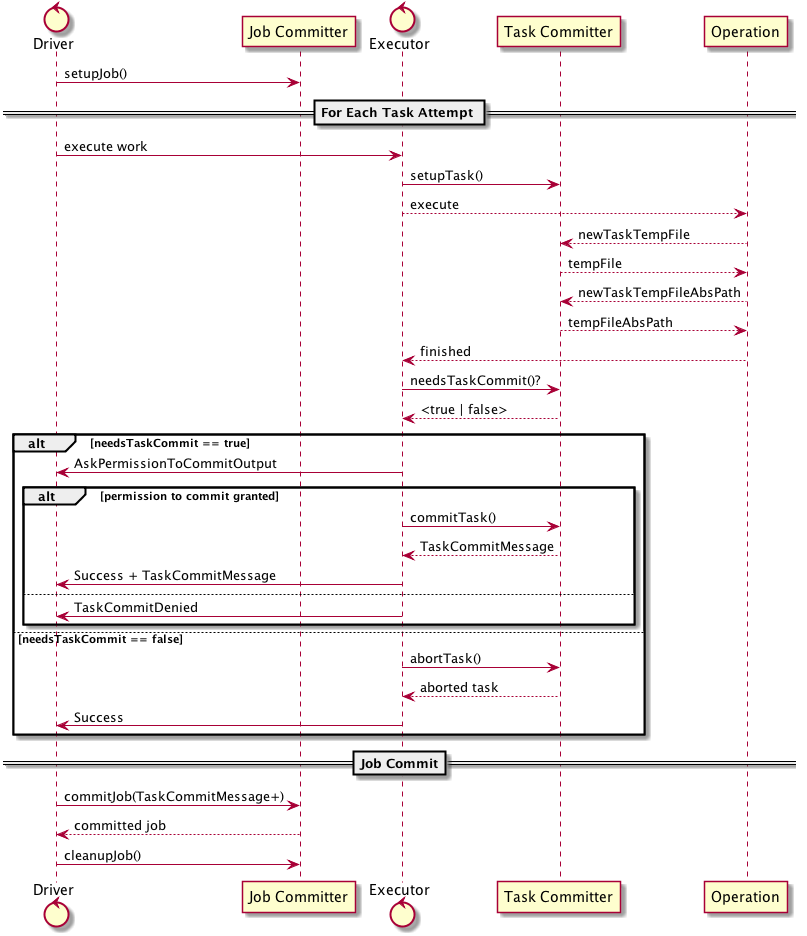
\includegraphics[width=.8\textwidth]{spark-protocol.png}
  \caption{Spark commit protocol)}
  \label{fig:spark-protocol}
\end{figure*}


A failure of an executor is detected (\TODO: how?);
all active tasks will be rescheduled.

As the failure may be a network partition, multiple task attempts may be active
simultaneously.

It is a requirement that no data is promoted until a task attempt is actually
committed.


Spark uses the Hadoop Committers within its commit protocol when
writing data to filesystems, but it is not restricted to only committing work
through the Hadoop APIs.

Again, it co-ordinates the commit operation between its drivers and executors
\footnote{Spark actually provides a hidden option to disable this
coordination\ \cite{SPARK-8029}; it is not clear if and how this is used.}.

Spark makes no attempt to recover from a failed job driver;
its mechanism for recovering from a failed job os "rerun the entire query".
What it does do is move the communication between operation and committer
from one of invoking the operation with an output directory to
that of permitting the operation to indirectly ask for a temporary file
and *a temporary file with a known destination*.

The simple temporary file operation, \texttt{newTaskTempFile()} is used
to request a temporary file.
The name of a file is constructed so as to match the final filename;
the committer which uses the Hadoop \texttt{FileOutputCommitter} places this
file in the task attempt directory.
As a result, the written file is committed through the same v1 or v2 algorithms
as with Hadoop.

The \texttt{newTaskTempFileAbsPath()} is a new operation.
This is needed to address the special case of Apache Hive, wherein
some parts of the data set are written to different locations than
under the destination directory of a job.
The operation, having calculated the absolute destination of the output,
requests a temporary file which will be placed in the final destination
directory on a job commit.

This is not supported in the Hadoop commit protocol.
Spark implements this operation atop the standard \texttt{FileOutputCommmiter}
as follows:

\begin{enumerate}
  \item An ``absolute path staging directory'' is created under the destination
  directory;
  this is \texttt{\_temporary-\$jobId}.
  \item When a new file with an absolute path is required, a path under this
  directory is generated, with a UUID in the filename.
  \item The mapping of absolute path to temporary file is stored in a map in the Task Committer.
  \item In the \texttt{commitTask()} operation, the map of all files to rename is passed back.
  \item In \texttt{commitJob()}, after invoking the Hadoop committer's \texttt{commitJob()}
  call, all files in the aggregate map of files to rename to absolute paths is iterated through.
  Each file is renamed(), in turn.
  \item Task abort will delete files of that task, while Job abort will delete
  the whole absolute path staging directory.
\end{enumerate}

This is extra operation is currently only used in that specific use case,
"Hive table with partitions elsewhere in the same filesystem as the active job".
This is not a common use case, at least with data stored in object stores.
Accordingly, our new committers do not support this operation
\footnote{It is possible to support this, but it would complicate cleaning up
after tasks, especially failed ones, and failed jobs.}.


% ========================================================================

\section{The Challenge of Object Stores}
\label{sec:object-stores}


\TODO: introduce object stores.

% As all filesystem
%operations are via the NameNode, all clients get a consistent view of the filesystem.
%And, as the


Object stores do not generally offer the full semantics of a filesystem.
Generally the set of operations available are an extended set of HTTP verbs:

\begin{description}[leftmargin=8em,style=nextline]
  \item[PUT] Atomic write of an object
  \item[GET] retrieve all or part of an object
  \item[HEAD] retrieve the object metadata
  \item[LIST] list all objects starting with a given prefix
  \item[COPY] copy a single object within the store
  \item[DELETE] Delete an object
\end{description}

There are usually two extra operations to address scale:
 a bulk delete call which may have partial failures,
and \emph{Multipart Upload}; a way to upload an object larger than 5GB\@.
The exact nature of multipart uploads varies from store to store.
For Amazon this is initiated as a sequence of POST calls, one to initiate,
one or more POST calls with data, and a final POST listing the (ordered)
etags of the uploaded object parts.
All but the last upload in the object must be 5 MB or larger


Object stores which lack an atomic $O(1)$ \texttt{rename()} operation cannot
be safely used as the direct destination of work from Apache Hadoop MapReduce
or Apache Spark, due to the existing ``Committer''s dependency upon rename for
atomic commit operations.
If the object store is eventually consistent, then even mimicing the \texttt{rename()}
operation is at risk of losing data.
Thus it is neither fast nor reliable.

% ========================================================================
\section{Integration with Hadoop and Spark}
\label{sec:integration}

A major challenge with this work is integrating the committers with Hadoop
and Spark, without making changes to their commit protocols themselves.

This was achieved by modifying the abstract class used for all data formats
which write to Hadoop filesystems, the \texttt{FileOutputFormat}, so that rather than
returning the standard \texttt{FileOutputCommitter}, it was possible to declare
a different committer factory for different filesystem schemas\ \cite{MAPREDUCE-6823}.
The \texttt{s3a:} schema is configured to refer to an S3A-specific factory, which
returns the specific S3A committer chosen on the job configuration.


As far as code integration is concerned, it is not entirely seamless, especially
with Spark, where we ultimately ended up creating a new spark committer for
writing the output, primarily to avoid exposing the new classes to the core
Spark codebase.

An alternative strategy would have been to retrofit an ``algorithm 3'' inside
the \texttt{FileOutputCommitter}, which would have implemented the plugin point.
This would have permitted the new committers to be inserted underneath any
subclass, so retrofit it to classes such as the \texttt{ParquetFileOutputCommitter}.
We chose not to do this

\begin{enumerate}
  \item The existing code is complex, containing two intermixed co-recursive
  algorithms.
  \item Our chages could unintentionally break the correctness of the existing committer.
  \item Subclasses of the existing committer must have been implemented to extend
  the protocol, perhaps by summarizing the output, writing extra files, etc.
  Changing the superclass behavior to not create output files until job commit
  ran the risk of breaking all this code.
\end{enumerate}

The factory design eliminated these risk at the expense of complicating
Spark/Parquet integration.

To address spark integration, we ultimately implemented two committers
The \texttt{PathOutputCommitProtocol}, which extended Spark's
\texttt{HadoopMapReduceCommitProtocol} class, relaxing the requirement of a
committer to be a subclass of \texttt{FileOutputCommitter}.

The \texttt{BindingParquetOutputCommitter} extends Parquet's
\texttt{org.apache.parquet.hadoop.ParquetOutputCommitter} class, relaying
all commit operations to that of whichever committer was committer dynamically created
through the factory mechanism.
This allows the requirement "Must be a ParquetOutputCommitter" to be satisfied
with any committer generated by a committer factory.

During the development of the committers, a change in Spark caused the
tests to fail.
Spark was enhanced to measure the amount of data created by a task, by
measuring the length of the written file\ \cite{SPARK-21669}.
With the Magic Committer, there is no written file, not until the job is committed.
Accordingly: the probe failed, so resulting in a task and, transitively a job, failure.
The Magic Committer was extended to create a zero-byte file in the expected path,
so guaranteed that the existence check will hold.
It does mean, however, that the statistics collected by Spark will not measure
the amount of data written.
A long term fix woud be to radically improve the means by which statistics are
collected by tasks and then aggregated in the job committer.
The latest versions of the HDFS and object store connectors are heavily instrumented,
collecting lots of information on filesystem client use.
for S3A this includes: times an HTTP1.1 connection was aborted on a file read,
the number of times a S3 request was throttled and retried,
even some latency statistics.
All of these would be useful if they could be collected by the job, aggregated
appropriately, and included in the job execution history.
It is possible to collect this information, and then pass this back.
Indeed, our committers do collect this data themselves, saving it in the
manifest files listing pending uploads, combinining this into the \SUCCESS file
in job commit.
This data is not yet extracted by the job committer and returned to the execution
environment.
This can be fixed.



% ========================================================================
\section{Correctness}\label{sec:correctness}

Do the two variant algorithms actually \emph{work}?


\subsubsection{Requirements of a valid commit algorithm}

First, a definition of correct behavior must be defined.

\begin{paragraph}
  \textbf{Completeness of output.}\\
  After a job has successfully returned from an invocation of \texttt{commitJob()},
  the destination directory tree will contain all files written under the output directory
  of all task attempts which successfully returned from an invocation of \texttt{commitTask()}.
  The contents of these files will contain exactly the data written by the user code.
  \emph{``You get what was committed''}
\end{paragraph}

\begin{paragraph}
  \textbf{Exclusivity of output.}\\
  After a job has successfully returned from an invocation of \texttt{commitJob()},
  the destination directory tree will contain *no* files written under the output directory
  of any task attempt which were not committed, or did not return from an invocation of \texttt{commitTask()}
  \emph{``And not what wasn't''}
\end{paragraph}

\begin{paragraph}
  \textbf{Continuity of correctness.}\\
  After a job has been successfully committed, no outstanding task may promote
  output into the destination directory.
  That is: if a task attempt has not ``failed'' mid-commit, merely proceeded at a slow rate,
  its output will not contaminate the directory of the already-successfull job.
  \emph{``A dead task stays dead''}
\end{paragraph}

\begin{paragraph}
  \textbf{Ability to abort safely.}\\
  If job attempt is aborted before \texttt{commitJob()}, is invoked, and
  \texttt{cleanupJob()} called, then the output of the attempt will not appear in the
  destination directory at any point in the future.
  \emph{``A cleanup up job is cleaned up''}
\end{paragraph}


The continuity of correctness requirement exludes that of a failed job.
We depend here upon the restriction that job will not commit its work unless
a heartbeat has been received in a predefined time interval from the YARN ResourceManager.
Assuming all clocks move forward at approximatly the same rate, if a job has
not committed nor received/responded to heartbeats outside that interval,
we can can conclude that the process will no longer commit work.
This failure to respond to heartbeats is what triggers YARN rescheduling a new
instance of the Job Manager and an attempt to kill the previous attempt.
A second Job attempt may conclude from the very fact that it has been launched
that the previous job attempt will not attempt to commit its work.


Not considered requirements are the following constrants:

\begin{itemize}
  \item The output of committed tasks not being present in the destination directory
  until the job is committed.
  Rationale: The v2 commit algorithm does not meet this requirement.

  \item That task commit operation is atomic.
  Rationale: The v2 commit algorithm does not meet this requirement.

  \item The job commit operation is atomic.
  Rationale: The v1 commit algorithm does not meet this requirement.

\end{itemize}

Having these as non requirements significantly simplifies implementations,
and allows for many different destinations of committed output to be supported.

The implication of not requiring these constraints is that the higher-level
commit protocol must react to failures or timeouts of the task and job
commit operations.
Nonatomic task attempt commit failures by failing the job. (v2)
Nonatomic job attempt commit failure by failing the job (v1).


We do attempt provide a formal proof of the correctness of the algorithms.
A TLA+ specification of the behavior of a consistent object store was created
during the process, however we have not completed that with the algorithm specifications.
Modelling an eventually consistent somewhat is somewhat challenging.

Informally, here is our assertions about the correctness of the two algorithms

\subsubsection{Correctness of the Staging Committer}

All task attempt output is written to the local filesystem;
it is implicity not in the destination object store until task commit.

In task commit, the contents of the local attempt directory are uploaded to the
destination, as incomplete uploads.
Hence: not visible until an operation completes the multipart upload.

The list of operations to complete is saved to the cluster filesystem, where
the V1 commit algorithm is used to commit this file.
The semantics of the V1 commit algorithm are used to guarantee that only
committed task attempt's output is promoted to the dataset of committed task
data, for the final job commit.

In the job commit, the V1 commit algorithm is used to commit that work, producing
a destination directory in the cluster filesystem listing all files generated
by committed task.
These are files containing the lists of pending commits.
As the V1 algorithm satisfies the completeness and exclusivity requirements,
we can be confident that reading in these lists will build an aggregate list
of files to commit, a list which is, transitively, complete and exclusive.

The final actions of the staging committer is to complete these uploads,
then cancel all other multipart uploads pending against the directory tree.
This will cancel the pending work of all tasks tasks which have uploaded staged
data, but which were not included in the list of committed tasks.

We can guarantee that neither this output *nor* that of any partitioned
task still uploading data, because that output will not be included in the
list of files promoted by the (now-completed) v1 commit process.

\subsubsection{Correctness of the Magic Committer}

This is harder to demonstrate, and depends on consistent directory
listings of the object stores, that is: all files created under a path
in the object store are visible to the LIST operation.
For Amazon S3, this requires a consistency layer, such as Semper or S3Guard
\ \cite{semper, S3Guard}.
The Magic committer was written and tested with the expecation that S3Guard
provides this.

All task attempt output is written to the object store, to the final (calculated)
destination.
However, they are not made visible until the job is committed.

The requirements of completeness and exclusivity must be met by
having the lists of pending uploads generated by committed task attempts propagated
to the Job Commit phase, and the list of pending uploads from uncommitted
attempts not propagated to the Job Commit.


Reviewing this code, there appears to be a small race condition in job commit,
wherein a task partitioned from the Job Manager during commitTask
(this considered failed and reattempted),
can still complete it's PUT of its list of uploads to commit, the ``pending set'',
overwriting that of the task attempt which had considered itself successful.
We cannot defense against that with the traditional strategy of creating
a file with overwrite=false, because against S3, there is no atomic
"create-no-overwrite" operation.
Instead we rely on the requirement of work, that any committed task attempt must
constitute a valid outcome, and argue that the pending set still constitues a valid
result from a task attempt.

It's notable that this process could be improved were the job commit
operation to supplied with a list of successful task attempts;
this would avoid inferring this state from the filesystem, except in
the case of job recovery from a commit algorithm capable of
rebuilding its state from a directory listing (i.e\ the v1 committer).


\TODO: HADOOP-15107

Regarding the requirement to abort safely, the fact that all writes are
not manifest until job commit means that the any writes from failed tasks
will remain ``pending''.

Data in this state is still billed by the megabyte, so must not be neglecte.
After the job commits all successful tasks it lists all outstanding
uploads against the destination directory and cancels them.
There are also command line tools to list and cancel pending uploads,
and, finally, it is possible to set a rule on an S3 bucket whereby uncompleted
pending uploads are deleted a specific time interval after their creation.
Our documentation recommends an interval of twenty-four hours here, to
clean out old data yet without affecting jobs ---assuming that all jobs
take less than a day to complete.


\subsection{testing}\label{subsec:testing}



Confidence in the correctness of the algorithms notwithstanding, there
is still the issue of the correctness of the implementation.


This was done through testing:

\begin{enumerate}
  \item Functional tests of the underlying IO operations against Amazon S3.
  \item Item tests of the commit operation against a mock S3 service endpoint.
  \item Invocations of the commit protocols in the normal and failing sequences of operations.
  \item Integration tests on a single host MapReduce cluster.
  \item Single-host integration tests of Spark integration, tests derived from Spark's own SQL test suites.
  \item Large scale integration tests in virtual test clusters.
  \item Peer review.
\end{enumerate}

To aid in demonstrating resilience to delayed consistency in object listing
operations and transient network failures, Hadoop's \texttt{hadoop-aws} module
now contains a special fault-injecting S3 connector: heavy throttling and
delayed consistency can both be simulated in the downstream tests, so
increasing confidence.

The large-scale integration tests have not, at the time of writing, highlighted any problems;
the simpler test suites were co-developed with the code, and exposing issues and
being expanded as new issues were discovered.
One bug the integration tests did show that our committers' cleanup code was
over-aggressive in listing and cancelling all outstanding uploads pending
on the destination directory.

Peer review is an integral part of the development process;
It was invaluable to have other developers interested in this problem
and willing to contribute time reviewing the code and testing it
in their own environments, including a commercial S3-compatible
storage system.

The \texttt{cleanupJob()} procedure used the existing S3A client command
\texttt{listMultipartUploads(directory)} to enumerate the updates,
which were then cancelled.
A detailed review of this code while trying to identify an intermittent problem
made clear that this existing routine had a long standing bug in it.
Rather than just list all uploads under a directory, it also included
all uploads in directories whose paths began with the same string.
That is, listing and cancelling pending work in the directory \texttt{/output/dataset1},
would also delete the output in \texttt{/output/dataset10}, \texttt{/output/dataset11/work},
...etc.
We are fortunate that this was found before the product shipped.
This does, however highlight our implementation's dependencies on the correctness
of the existing software, and how hard it is to imagine test cases which
can demonstrate the existence of bugs.
Who would have expected a test running in \texttt{/output/dataset1} to
cause an independent test in \texttt{/output/dataset10} iff the two tests
executions overlapped, and the first test executed is \texttt{cleanupJob()}
operation when the second had committed at least one task but not committed
the final job?


% ========================================================================

\section{Results}
\label{sec:results}


The performance of the new committers is not visible with small amounts
of data, as the number of HTTP requests is the dominant factor.
As the amount of data increases, the elimination of the copy operations
delivers a significant speedup to the new committers.
With a measured in-S3 copy time of ~6-10MB/s, the saving is 1 second per 10 MB
of data committed.

Comparing the staging and magic committers is interesting

The Staging committer writes all data locally, with the write bandwidth
of the local (usually virtual) disk.
In task commit, this data must be read and uploaded to the S3 service.
Usually it is the bandwdith between the server and S3 which is the bottleneck,
though as S3 throttles requests to specific shards, having many servers trying
to write to the same destination directory tree can slow down the write, irrespective
of bandwidth.
\ \cite{AWS-S3-throttling}.
If a single task has generated many files, or many tasks of the same job are
committing nearly simultaneously, this may be observed.
\footnote{Throttling can also be observed on read operations;
in such situations adding more workers is counterproductive.}

Job commit is a matter of reading the small `.pendingset` files saved in the
cluster filesystem (HDFS), and then issuing the relevant POSTs: one per uploaded
object.
This is parallelized, and not constrained by bandwidth.
Capacity in a local pool of HTTP1.1 connections, the time to create more,
and potentially throttling are the primary limits on IO performance at this point.

The Magic Committer uploads data in blocks as it is written: the larger
the amount of data created by a single task, the greater the performance
benefit over the Staging committer's task-commit-time upload.
However, task commit does list the task attempt directory and read all .pending
files within, an operation which can take a few hundred milliseconds per file,
and again, potentially throttled.
With only a single summary file written back, task commit is never
bandwidth constrained.

Job commit time is that of the Staging Committer, preceeded by a listing
of and reading in of the pending files of every committed task.
This is again a few hundred milliseconds per file, though parallelization
can reduce the delay.

Ignoring throttling, the magic committer is best with tasks which create
large amounts of data.
As well as avoiding the upload in the task commit, by reducing the
amount of storage needed in the virtual machine, VM and Container instances
with smaller amounts of storage can be request, or simply more tasks executed
per VM: computation, RAM and network bandwidth are the bottlenecks.

Protocol-wise, both committers meet the requirements of the Hadoop commit
protocol: no output visible until committed, and, as this materialization
takes place in job commit, it has better visibility characteristics than
the V2 algorithm.

One final feature to highlight is the "partitioned committer" variant
of the Staging Committer, which is designed to update an existing
dataset in-situ, only considering conflict with existing data in
those partitions for which data is actually generated.
This supports workflows where large datasets are updated on a daily basis,
without the need for any post-job copy of the new day's data into the
final dataset.
If the existing workflow for maintaining such large datasets involved
moving the new data into the aggregated dataset, those renames themselves
suffer from the performance constraints of the store's COPY operation.
Here, then, the speedup comes from the overall workflow, rather than
simply the query.





% ========================================================================

\section{Limitations}
\label{sec:limitations}

A key criticism of the new algorithm is that the job commit operation is not atomic;
it is $O(files)$ operation which may fail partway through.
We respond that as Hadoop's MapReduce V1 commit algorithm it itself non-atomic in job commit;
the job manager commit algorithm is designed to detect failures in job commits
of previous attempts, and either recover or fail, according to the actions
offered by the committer

A task process may exit without \texttt{abortTask()} being invoked.
Specifically, it exit immediately during the ping/response
heartbeat process if any of a number of conditions are met.

\begin{enumerate}
  \item Predefined task limits are exceeded
  (currently an optional limit on the number of bytes written to the local filesystem.
  \item Communications with the Job Manager have failed beyond configured limits.
  \item The reponse to the \texttt{ping()} call is \texttt{false}, indicating the current
  Job Manager does not consider the task to part of its set of active tasks.
\end{enumerate}

The first check is a defense against an errant process filling the local
filesystem with data;
the latter are symptoms of and reaction to different failures (loss of manager/network failure)
and restarted manager with no knowledge of active task, respectively.
There is also the without-warning failures triggered by the operating system
if limits on the execution environment are exceeded: usually memory allocation.

While OS-level failures can occur without warning, it would be useful if the
"managed" system exits triggered in the heartbeat thread were to invoke
an emergency task cleanup operation.
For the S3A committers, this would consist of aborting all pending uploads, and
deleting any local data.
While the Job committer's \texttt{cleanupJob()} operation is expected to clean up
the output of all task attempts, active participation of the tasks would
reduce the time incomplete uploads were pending (reducing costs) and
potentially free up local disk storage.

This appears to us to be an enhancement to the commit protocol which could
be considered.


One problem which may manifest itself in cloud-based deployments,
is that the Hadoop commit protocol assumes that time increases monotonically
on individual machines in the cluster.
The job manager and workers can use the interval between the last successful heartbeat
and the current time as the means by which they can consider themselves to have lost
contact with each other and system services.
In cloud environments clocks may stutter, proceed at significatly different rates,
and indeed, may even proceed backwards, especially if the VMs are moved between
physical cluster nodes.
We hope that Amazon's newly introduced \emph{Time Sync Service}
can address this on well-configured systems\ \cite{AWS-clock-service}.


% ========================================================================

\section{Related Work}
\label{sec:relatedWork}

Apache Spark (briefly) offered a zero rename committer,
the \emph{Direct Output Committer}.
With this committer, output was written directly to the destination directory;
both task and job commit operations were reduced to no-ops.
To avoid concurrency issues, speculative execution of tasks was automatically
disabled when this committer was used.
Unfortunately, the committer was still not resilient to failure: a failed
task could not be repeated, as its output was unknown.
For this reason it was discontinued \ \cite{SPARK-10063}.
It's absence is now noted by users, showing how a much zero-rename committer
was valued by users, even if it failed to offer any of the actual semantics
of a commit protocol.
Alternatively: performance is observable, whereas consistency and failures
are not considered important until they surface in production systems.

IBM's Stocator eliminates renames by also having a direct write to the
destination\ \cite{Stocator}.
As with the \emph{the Magic Committer}, it modifies the semantics of write
operations into the temporary directories of work, here the standard
\texttt{\_temporary} directory used by the classic \texttt{FileOutputCommitter}.
To avoid the failure semantics of Spark's \texttt{Direct Output Committer},
every remapped file is given a name which inserted the job and task attempt IDs,
while still preserving the sort order.
Failed and aborted tasks and jobs can then be cleaned up by their successors.
Stocator also generats a JSON-formatted \SUCCESS file, which offers
the ability to obtain a consistent list of the final files committed by a job,
even in the presence of listing inconsistency.

With this design, Stocator makes the output of work immediately visible;
there is no task commit, and the job commit is a matter of writing
the \SUCCESS file.

The actual implementation is achieved by misleading the classic committer,
changing the semantics of file creation under the task attempt diretories
under the \texttt{\_temporary} path.
The committer believes that it tasks are
 writing files to a temporary destination and renamining them, when
in fact they are being written direct to the final destination directory,
with a task-attempt-specific filename.

The rename operations of the the committer are then implicitly omitted:
there is no work to rename.

Note that Stocator's task commit operation is a no-op, thus repeatable.
Job commit is a listing of the output and generation of the manifest;
as the manifest PUT is atomic, the job commit itself is atomic.

What is critical for stocator is that the output of all failed tasks
is cleaned up, which is done in \emph{WHAT?}
This cannot be guaranteed in the failure case of: partitioned task
completing its commit after the job commit.
Thus our requirement "continuity of correctness" is not met.

The closest of the two S3A committers is the magic committer.
It too mosified the filesystem connctor to write the output to a
different destination than the path requested
in the user's code \texttt{createFile(path)} call.

However, the magic committer, does not attempt to mislead the existing committer,
instead we provide our own store-aware committer
Whch ensures that output is not actually manifest until
the final job is committed.
Thus it provides the standard semantics of task and job commmit: no data is
visible until the job is committed.

Could Stocator adopt a similar mechanism?
Perhaps: a \texttt{rename()} from a path in the \texttt{_temporary} directory
could be used to manifest an uncompleted write;
the latter would require the file write process to be modified as with
the magic committer.
`%One of the authors of this paper co-authored the Hadoop Openstack
%Swift committer atop which Stocator has been implemented ---they are not convinced
%that this would be possible, unless the Swift protocol has been extended.
`


\begin{table}
  \label{tab:other-committer-attributes}
  \begin{tabular}{ l c c }
    \hline
    & \textbf{Direct Committer} & \textbf{Stocator} \\
    Speculative Tasks & False & Delete task output \\
    Recoverable Job & False & False \\
    Abortable Job & Delete output & Delete output \\
    Observable & True & True \\
    Atomic Task Commit & True & True \\
    Idempotent Task Commit & True & True \\
    Atomic Job Commit & True & True \\
    Idempotent Job Commit & True & True \\
    \hline
  \end{tabular}
  \caption{Attributes of the Direct and Stocator committer algorithms}
\end{table}


The Direct Committer fails at the foundational requirement: ability to support
speculative or restarted task attempts.

Stocator also writes to the destination directory, but by renaming the output
files retains the ability to clean up the output of uncommitted tasks.
It does however, fail to meet our requirement ``Continuity of correctness.''

A task which is still in progress after the job commit will generate output
into the destination directory.


Neither committer is performing any operation in task commit other than creating
a \SUCCESS marker, which is both atomic and repeatable.


The key differences of the S3A committers are that the written files are
not observable in the destination directory tree until Job commit.
The classic file output committers postpone this until task (v2) or job (v1)
commit, and use rename as the low-cost operation to promote the files.


The Direct and Stocator committers avoid the rename, at the expense of making
the output visible even before job commit.

\begin{table}
  \label{tab:s3a-committer-attributes}
  \begin{tabular}{ l c c }
    \hline
    & \textbf{Staging Committer} & \textbf{Magic Committer} \\
    Speculative Tasks & True & True \\
    Recoverable Job & False & False \\
    Abortable Job & True & True \\
    Observable & False & False \\
    Atomic Task Commit & True & False \\
    Idempotent Task Commit & True & True \\
    Atomic Job Commit & False & False \\
    Idempotent Job Commit & False & False \\
    \hline
  \end{tabular}
  \caption{Attributes of the S3A committer algorithms}
\end{table}


The magic committer does aggregate the single `.pending` files describing
one written file into a per-task `.pendingset` file;
this is repeatable.
It is done purely to speed up job commit performance, as it reduces the
number of GET requests issued to be that of the number of committed tasks,
not the number of files.


The alternate strategy is move towards declaring the output of a job in
a manifest file, rather than implicitly defining it as ``all files in the directory
tree which do not begin with '.' or '\_'''.
The S3A committers and Stocator all generate manifest data in the defacto
standard \SUCCESS file.
For our committers, this was done initially for testing;
later it included the filesystem statistics of the process, so helping
collect data on IO costs.

Provided all relevant applications aggree to use a single, shared manifest
format, it may be possible to move to a simpler structure of
output being written straight to the destination, and the atomic PUT of the
manifest defining the output.


\section{Conclusions and Further Work}
\label{sec:conclusions}

Object Stores are becoming a common source and destination of data analysed
through Apache Hadoop and Spark.
The support for these stores manages to make them resemble filesystems in
terms of the API exposed to applications, so enabling existing code to
interact with the stores without modification.
However, the core semantics required by conventional commit algorithms, particulary
that of an $O(1)$ atomic rename, are not not met.
While the existing Hadoop/Spark commit algorithms appear to work, they lack
both the performance and correctness delivered when used with a "real" filesystem.

We have demonstrated that the use of object-store specific operations --here
the multipart PUT with its ability to complete the upload from a different host--
alow for object-store aware commit algorithms to be implemented,
algorithms which do meet these requirements.

The new Committers are implemented in Apache Hadoop 3.1, with a small bridging
library to aid integration with Apache Spark\ \cite{HADOOP-13786}.
We await the bug reports providing us with real-world deployment experiences
with excitement and trepidation.


These Committers have shown that the metaphor presented to applications,
\emph{Object Stores are File Systems} cannot be sustained.
As means of allowing existing applications to use stores as a source
of data the mimicing of directories and files works, albeit sometimes
inefficiently\ \cite{HADOOP-13208}).
What does not work is code which expects the strict semantics
offered by HDFS and other filesystems --atomic creation and rename algorithms.
This commit algorithm is one key example of a failure point, as
is any other algorithm attempting to use a shared filesystem
as a coordination mechanism between process.

The Hadoop project has long discussed the merits of explicitly
exposing an API for object stores, offering only the limited
set of verbs such stores present\ \cite{HADOOP-9565}.
However, we have been unable to progress because of the nuanced details
between the different stores\ \cite{S3, WASB, ADL, GCS}.
It is these nuances which prove critical in safely implementing
commit protocols and suchlike: any API which offered a lowest-common-denominator
would likely prove itself inadequate.

The integration with the Hadoop and Spark commit protocols is intended
to support different committers for different destination "filesystems".
We hope to see committers supporting other object stores, each
able to use store-specific operations.
What can be offered is common code for much of each implementation,
knowlege of the new algorithms needed, and
with the suites of tests used to validate their functionality.

One recurrent issue which this work has shown is that using the
filesystem or object store to communicate state from task attempts
to the job committer, and from the job committer to successor
applications, is brittle.

There is no reason why the job committer cannot be passedd the list of
successful task attempts from the job manager, as well as, ideally,
the list of failed attempts.
This can be used for the creation of a manifest, and for aiding cleanup
of failed task attempts.
The Spark commit protocol does permit committed task attempts to pass data
to the Spark committer;
use of this should be explored.



Finally, we note that the Hadoop commit protocols are woefully underdocumented;
understanding them involved stepping through tests with a debugger.
Given how critical the correctness of the protocol and committers and implementations
are, and how other projects depend also use the same code, there
are opportunities to better specify the protocol and APIs, and review
their use.

% ========================================================================

\section*{Acknowledgements}
\label{sec:acknowledgements}

% ========================================================================

\section{References}
\label{sec:references}

% Bibliography. Include

\bibliographystyle{IEEEtran}
\bibliography{bibliography.bib}


\end{document}
